\documentclass{article}
\usepackage[utf8]{inputenc}
\usepackage[greek,english]{babel}
\usepackage{alphabeta}
\usepackage{fancyhdr}
\usepackage{listings}
\usepackage{mathtools}
\usepackage{siunitx}
\usepackage{xcolor}
\usepackage{graphicx}
\usepackage{pgfplots}
\usepackage[export]{adjustbox}
\usepackage{biblatex}
\addbibresource{dl1-citations.bib}

%\pagestyle{fancy}
%\renewcommand\headrulewidth{0pt}
%\fancyhead{}
%\fancyfoot{}
%\fancyfoot[R]{\thepage}

\title{Εργαστηριακή Εργασία 1 - Λογικές Πύλες}
\author{Χρήστος Μαργιώλης - 19390133 \\ Τμήμα 8}
\date{Ιούνιος 2020}

\begin{document}

\begin{figure}[t!]
    \centering
    
\includegraphics[scale=0.3, center]{./res/Logo_University_of_West_Attica.png}
    \Large
    \textbf{Πανεπιστήμιο Δυτικής Αττικής} \\
    \large
    Τμήμα Μηχανικών Πληροφορικής και Ηλεκτρονικών Υπολογιστών \\
    Ψηφιακή Σχεδίαση
\end{figure}
\begin{figure}[b]
    \centering
    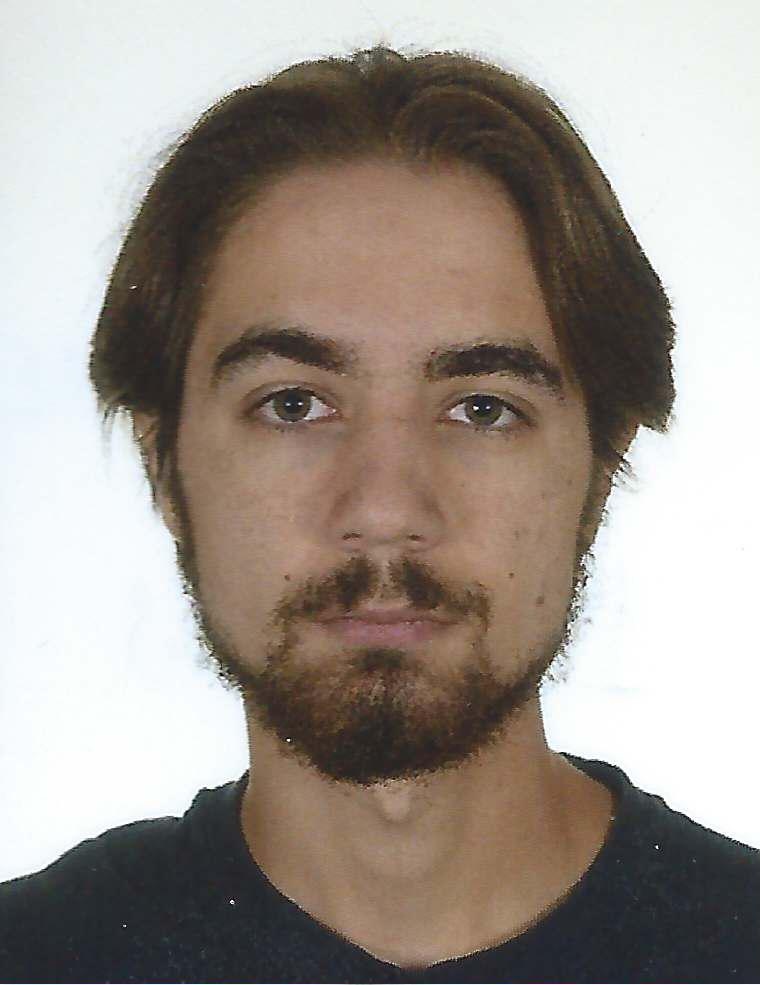
\includegraphics[scale=1]{./res/19390133.jpeg}
\end{figure}

\begin{titlepage}
\maketitle
\end{titlepage}

\renewcommand{\contentsname}{Περιεχόμενα}
\tableofcontents

\renewcommand{\abstractname}{Εισαγωγή}
\begin{abstract}
    Το αντικείμενο της εργασίας αυτής είναι η κατανόηση των λογικών πυλών,
    καθυστέρησης διάδοσης, μεγίστων/ελαχίστων επιτρεπόμενων ορίων τάσεων και ρευμάτων
    εισόδων/εξόδων, καθώς και της ικανότητας οδήγησης.
\end{abstract}
\pagebreak

\section{Συλλογή βιβλιογραφίας}
Η βιβλιογραφία που χρησιμποιήθηκε, αν και μικρή, κάλυψε τα βασικά προβλήματα της εργασίας.
Από την βιβλιογραφία πήρα πληροφορίες για την συμπεριφορά των λογικών πυλών.

\section{Περιγραφή υλοποίησης}
Για την υλοποίηση της εργασίας και βασισμένος στην παραπάνω βιβλιογραφία που συλλέχθηκε,
χρησιμποιήσα λογικές πύλες και εξισώσεις, πίνακες αλήθειας, καθώς και παλμογράφο για διάφορες
μετρήσεις.

\section{Θεωρητικό μέρος}
Λογικές πύλες είναι ψηφιακά κυκλώματα, τα οποία δέχονται μία ή παραπάνω δυαδικές
εισόδους και παράγουν μια δυαδική έξοδο. Τέτοιου είδους κυκλώματα τα περιγράφουμε με
την χρήση πινάκων αλήθειας και της άλγεβρας Boole. Οι λογικές πύλες με τις οποίες
θα ασχοληθούμε σε αυτή την εργασία είναι οι AND, OR, NAND, NOR, XOR, XNOR και NOT,
των οποίων η λειτουργία θα αναλυθεί στα αντίστοιχα κομμάτια \cite{efstathiou}.

\section{Εργαστηριακό μέρος}
\subsection{Πύλη AND}
\subsubsection{Περιγραφή}

Η πύλη AND δέχεται ως είσοδο δύο ή παραπάνω τιμές και παράγει έξοδο 1 μόνο αν
όλες οι είσοδοί της έχουν τιμή 1. Ο παρακάτω πίνακα αληθείας περιγράφει όλες
τις πιθανές καταστάσεις της πύλης AND.

\begin{center}
\begin{tabular}{|c|c|c|}
	\hline
	A & B & F \\
	\hline
	0 & 0 & 0 \\
	0 & 1 & 0 \\
	1 & 0 & 0 \\
	1 & 1 & 1 \\
	\hline
\end{tabular}
\end{center}

Η λογική εξίσωση της AND είναι $F = AB$

\subsubsection{Εφαρμογή στο Multisim}
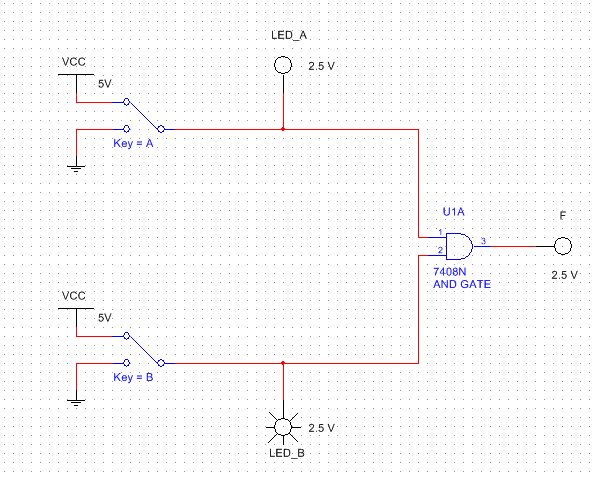
\includegraphics[width=\textwidth]{./res/and.png}

Στο παραπάνω κύκλωμα παρατηρούμε οτι τα LED που είναι συνδεδεμένα στις εισόδους
και στην έξοδο ανάβουν μόνο όταν ο διακόπτης είναι ανοιχτός, το οποίο μπορεί να
μεταφραστεί σε είσοδο 1. Στην συγκεκριμένη εικόνα ο μόνος διακόπτης ο οποίος είναι
ανοιχτός είναι αυτός της κάτω εισόδου, οπότε και το μοναδικό LED που θα ανάψει
είναι το LED\_B.  
Με βάση τον πίνακα αλήθειας της AND, αυτή είναι η περίπτωση που μόνο μία είσοδος είναι
1, το οποίο σημαίνει οτι ο διακόπτης της εξόδου δεν μπορεί να ανάψει, εφόσον δεν είναι
και οι δύο είσοδοι 1.

\subsection{Πύλη OR}
\subsubsection{Περιγραφή}

Η πύλη OR δέχεται ως είσοδο δύο ή παραπάνω τιμές και παράγει έξοδο 1 όταν τουλάχιστον
μία από τις εισόδους είναι 1. Ο παρακάτω πίνακα αληθείας περιγράφει όλες τις πιθανές
καταστάσεις της πύλης OR.

\begin{center}
\begin{tabular}{|c|c|c|}
	\hline
	A & B & F \\
	\hline
	0 & 0 & 0 \\
	0 & 1 & 1 \\
	1 & 0 & 1 \\
	1 & 1 & 1 \\
	\hline
\end{tabular}
\end{center}

Η λογική εξίσωση της OR είναι $F = A + B$

\subsubsection{Εφαρμογή στο Multisim}
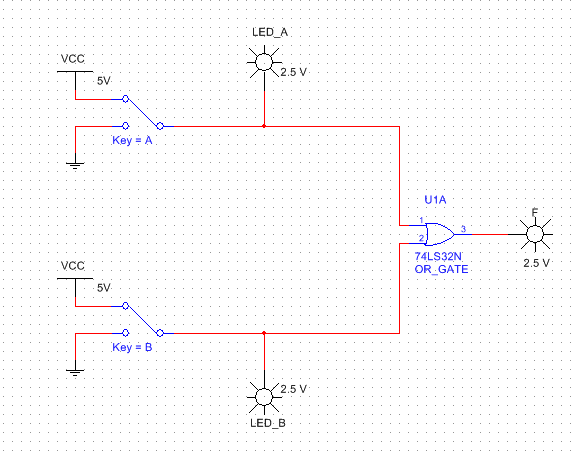
\includegraphics[width=\textwidth]{./res/or.png}

Όπως παρατηρούμε στο παραπάνω κύκλωμα, η πύλη OR δίνει έξοδο 1, και έτσι, το LED
που είναι συνδεδεμένο στην έξοδο ανάβει. Αυτό συμβαίνει γιατί στην προκειμένη
περίπτωση και οι δύο είσοδοι είναι 1. Η μοναδική περίπτωση για να μην ανάψει το LED
θα ήταν να είναι και οι δύο είσοδοι 0.

\subsection{Πύλη NAND}
\subsubsection{Περιγραφή}

Η πύλη NAND δέχεται δύο ή παραπάνω εισόδους και παράγει έξοδο 1 μόνο όταν και οι
δύο είσοδοι είναι 1. Η NAND, λόγω του ότι έχει συνδεδεμένη μία πύλη NOT στην έξοδό
της, αντιστρέφει οποιαδήποτε έξοδο θα παρήγαγε η AND. Ο παρακάτω πίνακα αληθείας
περιγράφει όλες τις πιθανές καταστάσεις της πύλης NAND.

\begin{center}
\begin{tabular}{|c|c|c|}
	\hline
	A & B & F \\
	\hline
	0 & 0 & 1 \\
	0 & 1 & 1 \\
	1 & 0 & 1 \\
	1 & 1 & 0 \\
	\hline
\end{tabular}
\end{center}

Η λογική εξίσωση της NAND είναι $F = \overline{AB}$

\subsubsection{Εφαρμογή στο Multisim}
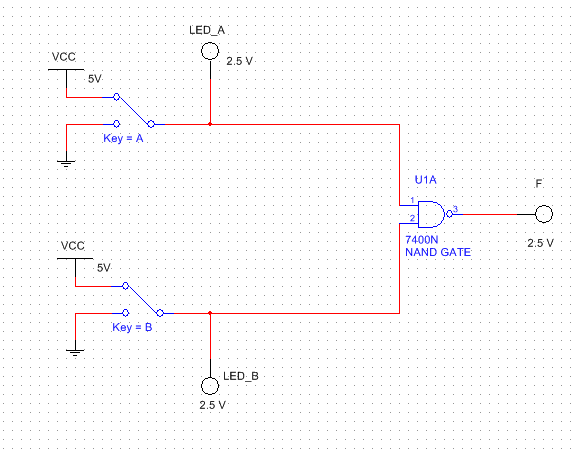
\includegraphics[width=\textwidth]{./res/nand.png}

Στο παραπάνω σχήμα παρατηρούμε ότι και οι δύο είσοδοι είναι 1, το οποίο με βάση
τον πίνακα αλήθειας της NAND είναι η μοναδική περίπτωση στην οποία η έξοδος είναι 0.
Έτσι, το LED σε αυτή την περίπτωση δεν ανάβει.

\subsection{Πύλη NOR}
\subsubsection{Περιγραφή}

Η πύλη NOR δέχεται δύο ή παραπάνω εισόδους και παράγει έξοδο 1 μόνο όταν και οι δύο
είσοδοί της είναι 0. H NOR παράγει την ακριβώς αντίθετη έξοδο από αυτή της OR λόγω της
πύλης ΝΟΤ που είναι συνδεδεμένη στην έξοδό της. Ο παρακάτω πίνακα αληθείας περιγράφει
όλες τις πιθανές καταστάσεις της πύλης NOR. 

\begin{center}
\begin{tabular}{|c|c|c|}
	\hline
	A & B & F \\
	\hline
	0 & 0 & 1 \\
	0 & 1 & 0 \\
	1 & 0 & 0 \\
	1 & 1 & 0 \\
	\hline
\end{tabular}
\end{center}

Η λογική εξίσωση της NOR είναι $F = \overline{A + B}$

\subsubsection{Εφαρμογή στο Multisim}
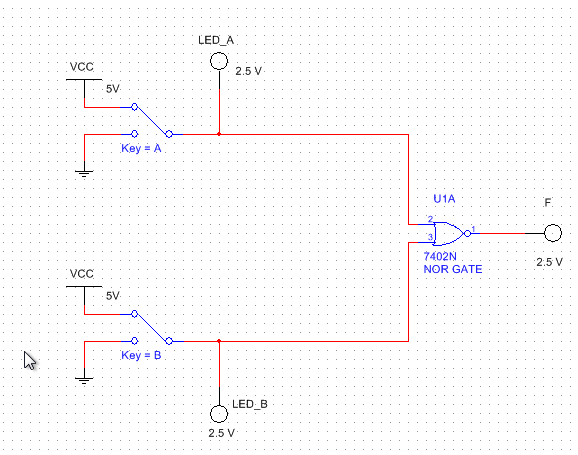
\includegraphics[width=\textwidth]{./res/nor.png}

Στο παραπάνω κύκλωμα παρατηρούμε ότι και οι δύο είσοδοι είναι 1, το οποίο με βάση
τον πίνακα αλήθειας της NOR σημαίνει ότι πρόκειται για την μοναδική περίπτωση που
η NOR θα παράξει έξοδο 0. Για αυτό τον λόγο το LED δεν ανάβει.

\subsection{Πύλη XOR}
\subsubsection{Περιγραφή}

H πύλη XOR δέχεται δύο ή παραπάνω εισόδους και παράγει έξοδο 1 μόνο όταν μία από τις
εισόδους της έχει τιμή 1. Ο παρακάτω πίνακας αληθείας περιγράφει όλες
τις πιθανές καταστάσεις της πύλης XOR.

\begin{center}
\begin{tabular}{|c|c|c|}
	\hline
	A & B & F \\
	\hline
	0 & 0 & 0 \\
	0 & 1 & 1 \\
	1 & 0 & 1 \\
	1 & 1 & 0 \\
	\hline
\end{tabular}
\end{center}

Η λογική εξίσωση της XOR είναι $F = A \oplus B = \overline{A}B + A\overline{B}$

\subsubsection{Εφαρμογή στο Multisim}
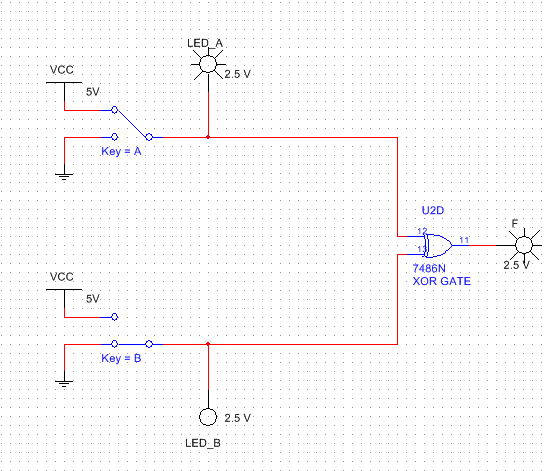
\includegraphics[width=\textwidth]{./res/xor.png}

Στο παραπάνω κύκλωμα παρατηρούμε ότι μόνο η μία από τις δύο εισόδους είναι 1, το οποίο
σημαίνει οτι πρόκειται για την περίπτωση που η XOR παράγει έξοδο 1. Για αυτό τον λόγο
ανάβει το LED που βρίσκεται στην έξοδο της XOR.

\subsection{Πύλη XNOR}
\subsubsection{Περιγραφή}

Η πύλη XNOR δέχεται δύο ή παραπάνω εισόδους και παράγει έξοδο 1 μόνο όταν οι είσοδοι
έχουν την ίδια τιμή. Η XNOR παράγει τις ακριβώς αντίθετες τιμές από αυτές που θα
παρήγαγε η XOR λόγω της πύλης NOT που είναι συνδεδεμένη στην έξοδό της. Ο παρακάτω
πίνακας αληθείας περιγράφει όλες τις πιθανές καταστάσεις της πύλης XNOR. 

\begin{center}
\begin{tabular}{|c|c|c|}
	\hline
	A & B & F \\
	\hline
	0 & 0 & 1 \\
	0 & 1 & 0 \\
	1 & 0 & 0 \\
	1 & 1 & 1 \\
	\hline
\end{tabular}
\end{center}

Η λογική εξίσωση της XNOR είναι $F = \overline{A \oplus B} = AB + \overline{AB}$

\subsubsection{Εφαρμογή στο Multisim}
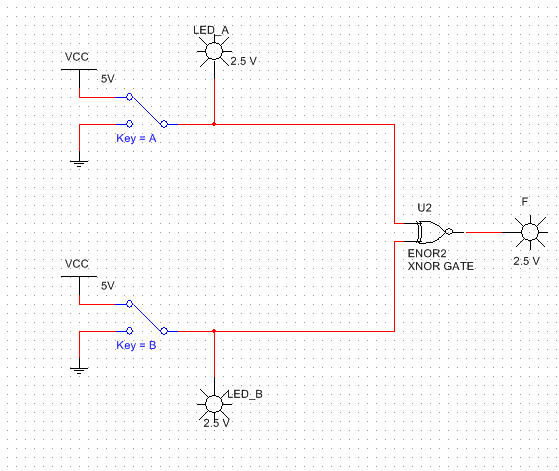
\includegraphics[width=\textwidth]{./res/xnor.png}

Στο παραπάνω σχήμα παρατηρούμε ότι και οι δύο είσοδοι είναι ίδιας τιμής, στην
προκειμένη περίπτωση 1, το οποίο σημαίνει οτι η έξοδος της XNOR θα είναι επίσης 1.
Για τον λόγο αυτό ανάβει το LED στην έξοδο της XNOR.

\subsection{Πύλη NOT}
\subsubsection{Περιγραφή}

Η πύλη NOT δέχεται μία είσοδο και αντιστρέφει την τιμή της. Ο παρακάτω πίνακας δείχνει
τις δύο πιθανές καταστάσεις που μπορούν να υπάρξουν.

\begin{center}
\begin{tabular}{|c|c|c|}
	\hline
	A & F \\
	\hline
	0 & 1  \\
	1 & 0  \\
	\hline
\end{tabular}
\end{center}

Η λογική εξίσωση της NOT είναι $F = \overline{A}$

\subsubsection{Εφαρμογή στο Multisim}
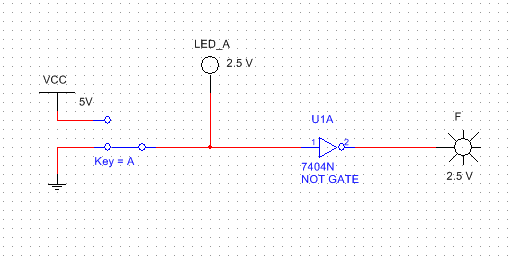
\includegraphics[width=\textwidth]{./res/not.png}

Στο παραπάνω κύκλωμα παρατηρούμε ότι η είσοδος είναι 0 και έτσι η NOT θα την
αντιστρέψει σε 1, και έτσι το LED θα ανάψει στην έξοδο της NOT.

\subsection{Έλεγχος ψηφιακών σημάτων από πύλες}

\begin{itemize}
	\item
	Πύλη AND \\
	\[A = 0 \Rightarrow F = 0\]
	\[A = 1 \Rightarrow F = B\]

	Με βάση τον πίνακα αλήθειας της AND, αν η είσοδος Α είναι 0, τότε η έξοδος F
	θα είναι πάντα 0, ασχέτως της τιμής του Β. Στην περίπτωση που το Α είναι 1, τότε
	η έξοδος είναι πάντα η ίδια με την τιμή του Β.

	Χρησιμοποιώντας την λογική εξίσωση της AND βλέπουμε ότι οι παραπάνω παραστάσεις
	επαληθεύονται αν θέσουμε τιμές στο Α. \\

	Για $A = 0$:
	\[F = AB \Rightarrow F = 0 \cdot B \Rightarrow F = 0\]

	Για $A = 1$:
	\[F = AB \Rightarrow F = 1 \cdot B \Rightarrow F = B\]

	\item
	Πύλη OR
	\[A = 0 \Rightarrow F = B\]
	\[A = 1 \Rightarrow F = 1\]

	Από την λογική εξίσωση της OR έχουμε ότι \\

	Για $A = 0$:
	\[F = A + B \Rightarrow F = 0 + B \Rightarrow F = B\]

	Για $A = 1$:
	\[F = A + B \Rightarrow F = 1 + B \Rightarrow F = 1\]

	\item
	Πύλη NAND
	\[A = 0 \Rightarrow F = 1\]
	\[A = 1 \Rightarrow F = \overline{B}\]

	Από την λογική εξίσωση της NAND έχουμε ότι \\

	Για $A = 0$:
	\[F = \overline{AB} \Rightarrow F = \overline{0 \cdot B} \Rightarrow
	F = 1 \cdot B \Rightarrow F = 1\]

	Για $A = 1$:
	\[F = \overline{AB} \Rightarrow F = \overline{1 \cdot B} \Rightarrow
	F = 0 \cdot B \Rightarrow F = \overline{B}\]

	\item
	Πύλη NOR
	\[A = 0 \Rightarrow F = \overline{B}\]
	\[A = 1 \Rightarrow F = 0\]

	Από την λογική εξίσωση της NOR έχουμε ότι \\

	Για $A = 0$:
	\[F = \overline{A + B} \Rightarrow\]
	Θεώρημα DeMorgan
	\[F = \overline{A} \cdot \overline{B} \Rightarrow F = \overline{0}
	\cdot \overline{B} \Rightarrow
	F = 1 \cdot \overline{B} \Rightarrow F = \overline{B}\]

	Για $A = 1$:
	\[F = \overline{A + B} \Rightarrow\]
	Θεώρημα DeMorgan
	\[F = \overline{A} \cdot \overline{B} \Rightarrow F = \overline{1}
	\cdot \overline{B} \Rightarrow
	F = 0 \cdot \overline{B} \Rightarrow F = 0\]

	\item
	Πύλη XOR
	\[A = 0 \Rightarrow F = B\]
	\[A = 1 \Rightarrow F = \overline{B}\]

	Από την λογική εξίσωση της XOR έχουμε ότι \\

	Για $A = 0$:
	\[F = A \oplus B = \overline{A}B + A\overline{B} \Rightarrow
	F = \overline{0} \cdot B + 0 \cdot \overline{B} \Rightarrow\]
	\[F = 1 \cdot B + 0 \cdot \overline{B} \Rightarrow
	F = B + 0 \Rightarrow F = B\]

	Για $A = 1$:
	\[F = A \oplus B = \overline{A}B + A\overline{B} \Rightarrow
	F = \overline{1} \cdot B + 1 \cdot \overline{B} \Rightarrow\]
	\[F = 0 \cdot B + 1 \cdot \overline{B} \Rightarrow
	F = 0 + \overline{B} \Rightarrow F = \overline{B}\]

	\item
	Πύλη XNOR
	\[A = 0 \Rightarrow F = \overline{B}\]
	\[A = 1 \Rightarrow F = B\]

	\[A \neq 0 \Rightarrow F = 0\]
	\[A = 1 \Rightarrow F = 1\]

	Από την λογική εξίσωση της XNOR έχουμε ότι \\

	Για $A = 0$:
	\[F = \overline{A \oplus B} = AB + \overline{AB} \Rightarrow\]
	Θεώρημα DeMorgan
	\[F = AB + \overline{A} + \overline{B} \Rightarrow
	F = 0 \cdot B + \overline{0} + \overline{B} \Rightarrow\]
	\[F = 0 + 1 + \overline{B} \Rightarrow F = (0 + 1) + \overline{B}
	\Rightarrow\]
	\[F = 1 + \overline{B} \Rightarrow F = \overline{B}\]

	Για $A = 1$:
	\[F = \overline{A \oplus B} = AB + \overline{AB} \Rightarrow\]
	Θεώρημα DeMorgan
	\[F = AB + \overline{A} + \overline{B} \Rightarrow
	F = 1 \cdot B + \overline{1} + \overline{B} \Rightarrow\]
	\[F = B + 0 + \overline{B} \Rightarrow F = (B + 0) + \overline{B}
		\Rightarrow\]
	\[F = B + \overline{B} \Rightarrow F = B\]
\end{itemize}

Πράγματι, τα παραπάνω αποτελέσματα επαληθεύονται και πειραματικά στο Multisim για
τα αντίστοιχα κυκλώματα, αλλά για λόγους χωρητικτότητας δεν μπορύν να υπάρχουν εικόνες
από το κάθε κύκλωμα.

\subsection{Καθυστέρηση διάδοσης}

Βάσει των μετρήσεων έχουμε ότι \\
\[t'_{PLH} = \si{56,818\ns}\]
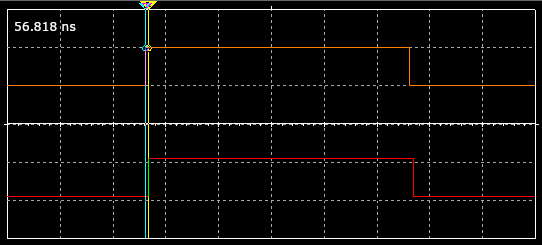
\includegraphics[width=\textwidth]{./res/tplh.png}
και
\[t'_{PHL} = \si{75,758\ns}\]
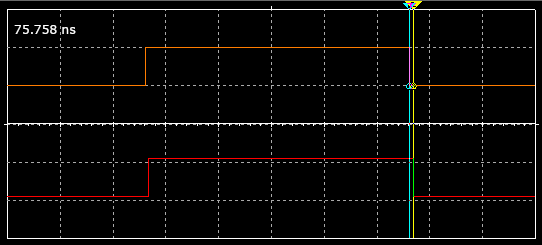
\includegraphics[width=\textwidth]{./res/tphl.png} \\

Για κάθε πύλη AND οι χρόνοι καθυστέρησης είναι \\
\[t_{PLH} = \frac{t'_{PLH}}{4} = \frac{\si{56,818\ns}}{4} = \si{14,205\ns}\]
\[t_{PHL} = \frac{t'_{PHL}}{4} = \frac{\si{75,288\ns}}{4} = \si{18,822\ns}\]

Ο μέσος χρόνος καθυστέρησης είναι \\
\[t_{PAV} = \frac{t_{PHL} + t_{PLH}}{2} = \si{\frac{18,822 + 14,205}{2}\ns} =
\si{16,513\ns}\] \\

Οπότε, ο πίνακας είναι
\begin{center}
\begin{tabular}{|c|c|}
	\hline
	$t'_{PLH}$ & $\si{56,818\ns}$ \\
	\hline
	$t'_{PHL}$ & $\si{75,758\ns}$ \\
	\hline
	$t_{PLH}$ & $\si{14,205\ns}$ \\
	\hline
	$t_{PHL}$ & $\si{18,822\ns}$ \\
	\hline
	$t_{PAV}$ & $\si{16,513\ns}$ \\
	\hline
\end{tabular}
\end{center}

\renewcommand\refname{Πηγές}
\printbibliography
\end{document}
